\documentclass[11pt,a4paper]{report}
\usepackage[utf8]{inputenc}
\usepackage[french]{babel}
\usepackage[T1]{fontenc}
\usepackage{amsmath}
\usepackage{amsfonts}
\usepackage{amssymb}
\usepackage{xcolor}

\usepackage{geometry}
\geometry{hmargin=2.5cm,vmargin=1.5cm}
\usepackage{wasysym}
\usepackage{graphicx}

\author{Mathieu Sarrat}
\title{LP6 - Premier Principe de la Thermodynamique}

\makeatletter
\renewcommand{\thesection}{\@arabic\c@section}
\makeatother


\begin{document}
\maketitle

\subsection{Pré-requis}
\begin{itemize}
	\item Vocabulaire de la thermodynamique : équilibre, transformations, variables d'état, 
	fonctions d'état, grandeurs extensives et intensives, température, pression, volume.
	\item Différentielle totale exacte et dérivées partielles.
	\item Théorème de l'énergie mécanique.
\end{itemize}

\subsection{Objectifs}

\newpage
\section{Introduction}

La thermodynamique, née au début du $\text{XIX}^\text{ème}$ siècle en pleine Révolution Industrielle, est la science qui étudie la transformation et les échanges d'énergie à l'échelle macroscopique (systèmes constitués d'un grand nombre de constituants élémentaires). Cette époque est une période de bascule pour les sciences, durant laquelle on passe progressivement d'une vision continue de la matière (la lumière, l'électricité et la chaleur sont vues comme des fluides) à la vision moderne (matière granulaire : atomes, molécules). Parfois la technique se développe plus vite que la théorie : la thermodynamique a originellement été développée pour établir la relation entre les phénomènes mécaniques et les phénomènes thermiques mis en jeu lors du fonctionnement de machines thermiques déjà construites et fonctionnelles (la première machine à vapeur a été inventée par Denis Papin en 1707, alors que les principes de la thermodynamique n'ont pas été énoncés avant la première moitié du $\text{XIX}^\text{ème}$ siècle, soit un siècle plus tard). L'étude théorique de la thermodynamique repose sur quelques principes fondamentaux, qui ne sont pas démontrables et sont juste le résultat de l'expérience. Comme on ne leur connaît pas de contre-exemple, ils sont considérés comme fondés. Le Premier Principe de la Thermodynamique est celui de la conservation de l'énergie d'un système.

Nous avons déjà mentionné, en mécanique, la conservation de l'énergie mécanique d'un système soumis à des forces dites conservatives (que l'on peut écrire à partir d'une énergie potentielle et dont le travail fourni ne dépend pas du mouvement effectué). Le théorème de l'énergie mécanique, s'il peut être d'une aide précieuse pour étudier de nombreux phénomènes, n'est cependant pas capable d'expliquer certaines situations pourtant fréquentes.

Où va l'énergie cinétique d'une main en mouvement exerçant un frottement sur une surface solide qui reste immobile ? L'expérimentateur, s'il frotte trop vite et trop fort, sentira rapidement une sensation de brûlure : il y a transformation d'énergie cinétique en énergie thermique. L'Homme préhistorique frottait deux bouts de bois pour créer du feu (en provoquant une réaction chimique de combustion du bois). Ce dernier exemple permet de souligner que la thermodynamique ne se limite pas à la mécanique et à la thermique. On sait que certaines réactions chimiques produisent une élévation de température du milieu réactionnel. On sait aussi qu'un conducteur électrique parcouru par un courant dégage de la chaleur. On sait qu'il est possible de convertir de l'énergie mécanique en énergie électrique, et vice versa. Lors du siècle dernier, la thermodynamique a été utilisée pour établir des modèles expliquant certains phénomènes (la supraconductivité, par exemple) sans toutefois permettre leur compréhension d'un point de vue microscopique.

Nous commencerons par développer la notion d'énergie totale d'un système physique. Nous énoncerons ensuite le Premier Principe de la Thermodynamique et l'appliquerons à quelques situations physiques.



\newpage
\section{\'Enoncé et compréhension du premier principe}

\subsection{Rappel sur la notion de système en thermodynamique}

\begin{itemize}
	\item \textbf{Système} $\equiv$ portion de l'espace contenue à l'intérieur d'une surface fermée $\mathcal{S}$
	\item \textbf{Milieu extérieur} $\equiv$ tout ce qui est à l'extérieur de $\mathcal{S}$
	\item \textbf{Paroi} $\equiv$ la surface fermée $\mathcal{S}$, qui n'est pas considérée comme matérielle (c'est un trait d'épaisseur infiniment fine)
	\item \textbf{Univers} $\equiv$ Système $+$ Milieu extérieur.\\
\end{itemize}

\begin{figure}[h!]
\begin{center}
	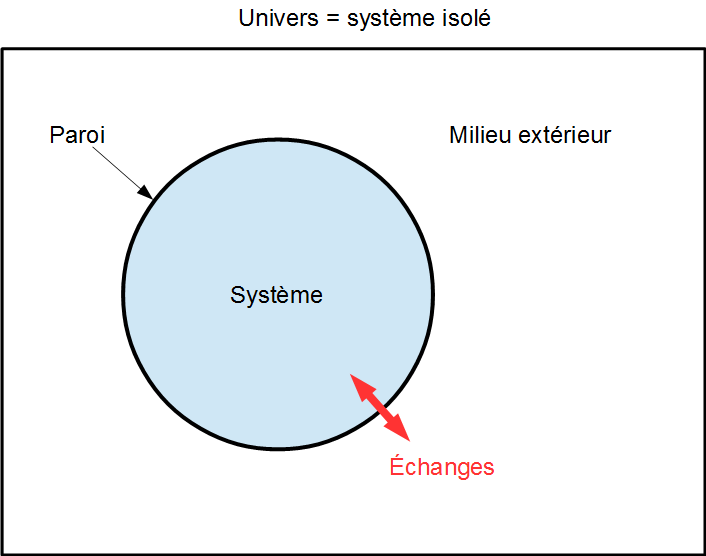
\includegraphics[scale = 0.3]{systeme.png}
	\caption{Vision de l'univers en thermodynamique.}
	\label{fig:systeme}
\end{center}
\end{figure}

Un système peut échanger avec le milieu extérieur à travers la paroi et en fonction de la nature de cette paroi. Elle peut être virtuelle ou réelle, elle peut laisser passer de la matière, de l'énergie, les deux ou rien du tout. On distingue trois cas :
\begin{itemize}
	\item le système ne peut échanger ni matière, ni énergie : \textbf{système isolé} ($\neq$ système mécaniquement isolé).
	Exemple : l'univers thermodynamique
	\item le système peut échanger de l'énergie, mais pas de matière : \textbf{système fermé}.
	Exemple : tout récipient fermé dont les parois sont imperméables.
	\item le système peut échanger de l'énergie et de la matière : \textbf{système ouvert}.
	Exemple : être vivant, fusée, une pièce dans une maison ou un petit volume d'air (mais contenant suffisamment de particules) dans cette pièce.\\
\end{itemize}

Un système est caractérisé par son nombre de particules $N$, son énergie totale $E$, et par un certain nombre de variables d'état comme la température $T$ ou le volume $V$.\\

On se limitera, dans cette leçon, au cas des systèmes isolés et fermés : seuls des échanges d'énergie sans transfert de matière nous intéressent.

\subsection{Principe de conservation de l'énergie}

\begin{itemize}
	\item \'Enoncé en 1845 par von Mayer : \textcolor{red}{"l'énergie totale d'un système isolé se conserve."}\\
	
	\item L'énergie totale $E$ est donc une grandeur conservative : elle ne peut pas être créée ou détruite.\\
	
	\item Pour un système fermé, la variation d'énergie totale est telle que :
	\begin{equation}
		\Delta E = E^r,
	\end{equation}
	où $E^r$ est la quantité d'énergie échangée entre le système et le milieu extérieur. Ces échanges peuvent se faire sous deux forme : travail $W$ et chaleur $Q$, ainsi
	\begin{equation}
		\Delta E = W + Q.
	\end{equation}
\end{itemize}

Avant d'énoncer le Premier Principe de la Thermodynamique, il nous faut préciser ce qu'est l'énergie totale.

\subsection{\'Energie totale et énergie interne}

Soit $E$ l'énergie totale du système. On définit \textbf{l'énergie interne} $U$ du système comme
\begin{equation}
	U \equiv E - E_{k}^{\text{macro}} - E_{p}^{\text{macro}}.
\end{equation}

L'énergie interne est \textbf{l'énergie qu'il reste} lorsqu'on soustrait à l'énergie totale :
\begin{itemize}
	\item son énergie cinétique $E_{k}^{\text{macro}}$ à l'échelle macroscopique,
	\item son énergie potentielle $E_{p}^{\text{macro}}$ liée aux forces s'exerçant depuis le milieu extérieur.
\end{itemize}
Formulé autrement, l'énergie interne correspond à l'énergie totale du système (énergie mécanique définie à partir de l'échelle microscopique), à laquelle on retire l'énergie mécanique calculée à l'échelle macroscopique. Dans le cas d'un corps macroscopiquement au repos, il reste :
\begin{equation}
	U = E.
\end{equation}

L'énergie interne, présentée comme ci-dessus, est une sorte de \textbf{boîte noire} permettant de prendre en compte tout ce que la mécanique seule ne peut pas faire de façon simple. Il faut se rendre compte que les notions d'atome et de molécule faisaient encore débat et s'installaient tout doucement dans les idées à l'époque où la thermodynamique a été construite (on parlait surtout d'hypothèse atomique). Beaucoup imaginaient encore la matière comme un continuum : la thermodynamique est une science macroscopique et on se placera dans ce cadre simplifié pour tout le reste de la leçon.\\

Avant d'aller plus loin, essayons tout de même de préciser la notion d'énergie interne. On peut distinguer deux formes d'énergie pour tout type de système :
\begin{itemize}
	\item énergie cinétique, liée au mouvement du "système dans son ensemble" (mouvement du centre de masse pour un solide indéformable, champ des vitesses pour un matériau fluide) et au mouvement des particules qui le constituent
	\item énergie potentielle, liée à l'interaction entre le système et des champs électrique, gravitationnel ou magnétique provenant du milieu extérieur, mais aussi aux interactions entre les molécules, ions, atomes, électrons, noyaux et nucléons qui le constituent.
\end{itemize}
On peut distinguer deux types de contributions pour chacune de ces deux catégories :
\begin{itemize}
	\item une contribution \textbf{macroscopique}, accessible à nos sens, correspondant à l'énergie cinétique macroscopique $E_{k}^{\text{macro}}$ du système en mouvement dans son référentiel d'étude, et aux énergies potentielles $E_{p}^{\text{macro}}$ du système placé dans un champ (de gravitation, électrique ou magnétique).
	\item une contribution \textbf{microscopique}, imperceptible pour nous dans ses détails, correspondant à l'énergie cinétique d'agitation thermique des particules et aux énergies potentielles relatives aux interactions microscopiques entre les constituants de la matière : énergies potentielles de liaison chimique, interactions de Van der Waals, interactions nucléaires ...\\
\end{itemize}

Prenons un exemple concret pour illustrer tout ça : soit une grosse quantité d'eau transportée dans un camion citerne en déplacement sur une route :
\begin{itemize}
	\item l'eau se déplace dans son ensemble, du fait du mouvement du camion. De plus, la route n'étant ni droite, ni plane, on imagine fort bien qu'elle est agitée. Ces deux types de mouvement contribuent à l'énergie cinétique dite macroscopique. On peut se débarrasser de la première contribution en se plaçant dans le référentiel du camion, mais celle liée à la déformation du fluide est toujours là;
	\item l'eau est bien entendu soumise à son poids, ce qui est modélisé par une énergie potentielle de pesanteur, elle aussi macroscopique;
	\item l'eau est à température ambiante : les molécules d'eau bougent par agitation thermique, indépendamment du fait que le camion et le fluide soient en mouvement. Ce mouvement contribue à l'énergie cinétique microscopique;
	\item les molécules d'eau interagissent entre elles en formant des liaisons hydrogène et via des interactions de type Van der Waals. Au sein d'une molécule, les électrons de valence participent à des liaisons covalentes, les électrons de coeur sont liés à l'atome par l'interaction électromagnétique. Les nucléons d'un atome d'O sont liés par interaction forte. Toutes ces interactions contribuent à l'énergie potentielle microscopique.\\
\end{itemize}

L'énergie interne est en fait une \textbf{modélisation macroscopique (une moyenne) de l'énergie relative aux processus microscopiques} intervenant dans le système, phénomènes qui n'étaient pas bien ou pas du tout connus jadis.

\subsubsection{Propriétés de l'énergie interne}
\begin{itemize}
	\item $U$ est une \textbf{fonction d'état}. Sa variation ne dépend que de l'état initial et que de l'état final. Elle ne dépend pas du type de transformation, ni de la rapidité avec laquelle celle-ci a lieu. Si le système peut être décrit macroscopiquement de façon univoque à partir de sa température et de son volume, la variation $dU$ au cours d'une transformation infinitésimale est une différentielle totale exacte et elle s'écrit
	\begin{equation}
		dU = \left(\frac{\partial U}{\partial T}\right)_V dT + \left(\frac{\partial U}{\partial V}\right)_T dV.\\
	\end{equation}
	Cette propriété sera très utilisée : lorsqu'on ne connaît pas la transformation réelle ou qu'on ne sait pas la modéliser, on peut toujours imaginer une ou plusieurs 			transformations fictives reliant l'état initial et l'état final. La variation d'énergie interne le long de cette série de transformations fictives sera égale à celle 			obtenue avec la transformation réelle. Notons enfin que la variation de $U$ sur une transformation cyclique (l'état initial et l'état final sont identiques) 
	est forcément nulle : $\Delta U_{cycle} = 0$.\\
	
	\item $U$ est une grandeur \textbf{supposée extensive}. Si le système 1 a une énergie interne $U_1$, et que le système 2 a une énergie interne $U_2$, alors la réunion des systèmes 1 et 2 aura une énergie $U_1$ + $U_2$. Ceci est \textbf{rigoureusement faux} (sauf pour un mélange de deux gaz parfaits, puisqu'il n'y a pas d'interaction entre molécules d'un gaz parfait), mais peut être approximativement considéré comme vrai si les constituants des systèmes 1 et 2 interagissent peu entre eux (gaz très dilués).\\
	
	\item $U$ est \textbf{indépendante du référentiel} dans lequel elle est étudiée.
\end{itemize}

\subsection{\'Enoncé du Premier Principe}

Le Premier Principe de la Thermodynamique \textbf{découle du principe de conservation de l'énergie}.

\'Enonçons le pour un système fermé :\\
\textcolor{red}{"Il existe une fonction d'état U, appelée énergie interne, telle qu'au cours d'une transformation quelconque d'un système fermé :
\begin{equation}
	\Delta E_{k}^{\text{macro}} + \Delta E_{p}^{\text{macro}} + \Delta U = W + Q
\end{equation}
}
Si le système est macroscopiquement au repos, on a
\begin{equation}
	\Delta U = W + Q,
\end{equation}
qui est la formulation que nous retiendrons pour le restant de ce cours.\\

Pour une \textbf{transformation infinitésimale}, on écrira :
\begin{equation}
	dU = \delta W + \delta Q.
\end{equation}
On n'écrit pas $dW$ ou $dQ$ car $W$ et $Q$ ne sont pas des fonctions d'état. Le travail et la chaleur ne caractérisent pas l'état d'un système, ce sont des façons d'échanger de l'énergie. $\delta Q$ et $\delta W$ ne sont pas des variations de travail ou de chaleur mais des quantités d'énergie échangées sous forme de travail et de chaleur. Leur somme est cependant équivalente à une variation de fonction d'état. Nous allons détailler les notions de travail et de chaleur un peu plus loin.

\subsubsection{Remarque 1 : système isolé}
Dans le cas d'un système isolé, l'énergie interne est conservée, puisque le système est incapable de gagner ou de recevoir de l'énergie. Il en découle que, pour toute transformation :
\begin{equation}
	\Delta U = 0.
\end{equation}

\subsubsection{Remarque 2 : transformation cyclique}
L'énergie interne est une fonction d'état. Une transformation cyclique (qui part d'un état A pour revenir au même état A) implique une variation totale nulle de $U$ :
\begin{equation}
	\Delta U_{\text{cycle}} = 0 = W_\text{cycle} + Q_\text{cycle} \Rightarrow W_\text{cycle} = - Q_\text{cycle}.
\end{equation}
Le travail fourni à un système macroscopiquement au repos lors d'une transformation cyclique est intégralement dégradé en chaleur et vice-versa. Attention, le Premier Principe permet d'évaluer les échanges de chaleur et de travail au cours d'une transformation, mais il ne dit rien au sujet de la faisabilité de cette transformation. C'est au Second Principe de la Thermodynamique qu'incombe ce rôle.

\subsubsection{Remarque 3 : définition d'un principe}
Un principe est une loi physique qui n'a pas été démontrée, mais qui n'est pas invalidée pour autant par l'expérience.

\subsubsection{Remarque 4 : choix des variables}
On montrera dans une autre leçon que la variation d'énergie interne s'exprime de façon privilégiée en fonction des variations d'entropie $S$ et de volume $V$. Ainsi, on a l'\textbf{identité thermodynamique}.
\begin{equation}
	dU = TdS - pdV.
\end{equation}
Le Premier Principe est toujours vérifié :
\begin{equation}
	dU = \delta Q + \delta W,
\end{equation}
mais on ne peut pas identifier terme à terme ces deux expressions dans le cas général pour une transformation réelle. En effet $\delta Q = T dS$ et $\delta W = - pdV$ ne sont \textbf{vraies que pour} une transformation \textbf{quasi-statique réversible}.

\newpage
\section{Transformations d'un système fermé et nature des échanges}

\subsection{\'Echange d'énergie par travail}

Le travail est une grandeur intimement liée à la notion de force. Une force $\bold{F}$ exercée sur un objet matériel qui se déplace de $d\bold{r}$ lui fournira un travail
\begin{equation}
	\delta W = \bold{F}\cdot d\bold{r}.
\end{equation}

Intéressons-nous au travail des forces de pression qui s'exercent sur la paroi du système. En déformant cette paroi, ces forces peuvent comprimer ou dilater le système, ce qui correspond pour celui-ci à un gain ou à une perte d'énergie sous forme de travail. En l'absence de variation de volume, les forces de pression ne travaillent pas. Pour modéliser ceci, imaginons du gaz contenu dans un récipient cylindrique dont le volume peut varier grâce au déplacement d'un piston.

\begin{figure}[h!]
\begin{center}
	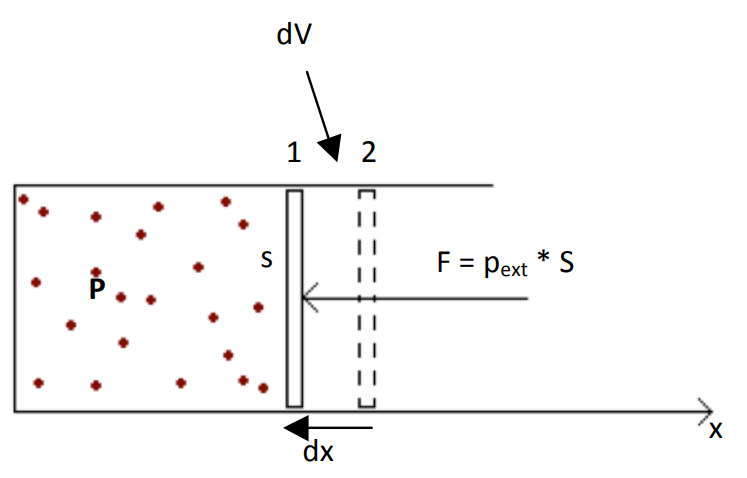
\includegraphics[scale = 0.35]{travail_pression.png}
	\caption{Travail des forces de pression pour un piston.} 
	\label{fig:travail_pression}
\end{center}
\end{figure}

La pression extérieure est notée $p_{ext}$. Le piston a une section $\mathcal{S}$ et sa position est repérée par $x$.
La force de pression exercée par le piston s'écrit
\begin{equation}
	\bold{F} = -p_{ext}\mathcal{S}\bold{e}_x,
\end{equation}
et $d\bold{r} = dx \bold{e}_x$ ($dx$ négatif sur le schéma)
d'où 
\begin{equation}
	\delta W = - p_{ext}\mathcal{S}dx. 
\end{equation}
Si $V = \mathcal{S}x$ le volume du gaz, la variation de volume est $dV = \mathcal{S}dx$, d'où
\begin{equation}
	\delta W = - p_{ext}dV.
\end{equation}
Sur le schéma, $dx <0$ donc $dV <0$ donc $\delta W > 0$ : le gaz gagne de l'énergie sous forme de travail lorsqu'on le comprime.
Pour la transformation totale,
\begin{equation}
	W = \int\delta W = -\int p_\text{ext}dV.
\end{equation}
C'est bien la pression extérieure qui figure sous l'intégrale. La pression du gaz $p$ n'est définie que pour un état d'équilibre, autrement dit au début $p = p_i$ et à la fin $p = p_f$ de la transformation. Son existence en tant que variable d'état au milieu d'une transformation n'est pas garantie (c'est une variable intensive), puisque la présence d'états d'équilibre durant la transformation ne l'est pas.

\subsubsection{Cas particuliers}
Le travail reçu par le système dépend du type de transformation qu'il subit. Voyons comment le travail $W$ reçu par le système s'écrit pour plusieurs types de transformations
\begin{itemize}
	\item \textbf{transformation quasi-statique} (succession d'états d'équilibres infiniment proches, donc, à tout instant de la transformation, 
	$p_\text{ext} = p$, $p$ étant la pression du gaz dans le système\footnote{On a également $T_\text{ext} = T$ à chaque instant sinon il ne peut pas y avoir d'équilibre. 
	Ce type d'égalité se généralise à toute variable intensive décrivant le système.}) :
		\begin{equation}
			\delta W = -p dV \Rightarrow W = \int\delta W = -\int p dV,
		\end{equation}
		mais $p$ varie lors de la transformation (une transformation quasi-statique n'est qu'une idéalisation, 
		le déséquilibre est nécessaire pour qu'il y ait transformation) donc il reste sous l'intégrale. On doit donc trouver une relation entre $p$ et $V$ pour mener le 				calcul à terme. Dans le cas d'un gaz parfait, l'équation d'état $PV = nRT$ et la température $T$ sont vérifiée/définie puisque la transformation est quasi-statique. 
		Si de plus cette transformation est isotherme($T$ constante à chaque instant de la transformation), on a
		\begin{equation}
			\delta W = -\int nRT\frac{dV}{V} \Rightarrow W = - nRT\int \frac{dV}{V} = + nRT \text{ln}\left(\frac{V_i}{V_f}\right).
		\end{equation}
	\item \textbf{transformation à pression extérieure constante} 
		\begin{itemize}
			\item monobare $p_\text{ext} = p_{i} = p_f$ : équilibre mécanique assuré en début et en fin de transformation seulement.
			\item isobare $p_\text{ext} = p$ à tout instant de la transformation : équilibe mécanique assuré tout le long de la transformation
		\end{itemize} )
		\begin{equation}
			\delta W = -p_\text{ext}\int dV \Rightarrow \Delta W = -p_\text{ext}\Delta V.
		\end{equation}
	\item \textbf{transformation isochore} $dV = 0$ à chaque instant de la transformation, donc
		\begin{equation}
			\delta W = 0 \Rightarrow W = 0.
		\end{equation}
\end{itemize}

\subsubsection{Variation de U lors d'une transformation adiabatique}

Une transformation adiabatique est telle que $\delta Q = 0$ pour toute transformation élémentaire constituant la transformation totale, d'où
\begin{equation}
	dU = -p_\text{ext}dV \Rightarrow \Delta U = -\int p_\text{ext}dV,
\end{equation}
où l'intégrale peut être calculée comme au paragraphe précédent, selon que la pression extérieure est constante ou non, que la transformation est quasi-statique ou non.

\subsection{\'Echange d'énergie par chaleur et coefficients calorimétriques}

La chaleur est définie comme la quantité d'énergie qu'il faut ajouter au travail reçu lors d'une transformation pour obtenir l'échange total d'énergie. Ainsi,
\begin{equation}
	Q \equiv E^r - W = \Delta U - W
\end{equation}
pour un système macroscopiquement au repos. Elle s'exprime en Joule (J), tout comme le travail.\\

On parle d'échange thermique lorsqu'un système échange de la chaleur avec le milieu extérieur. En l'absence d'échange thermique, $Q = 0$ et la transformation est dite adiabatique. On peut réaliser une telle transformation en intercalant une paroi empêchant tout transfert thermique entre le système et le milieu extérieur.

\subsubsection{Variation de U lors d'une transformation isochore}

Nous avons vu que, lors d'une transformation infinitésimale,
\begin{equation}
	dU = \left(\frac{\partial U}{\partial T}\right)_V dT + \left(\frac{\partial U}{\partial V}\right)_T dV.\\
\end{equation}

Supposons cette \textbf{transformation isochore} ($dV = 0$ car volume constant tout au long de la transformation). La relation précédente s'écrit 
\begin{equation}
	dU = \left(\frac{\partial U}{\partial T}\right)_V dT.\\
\end{equation}

En outre, le travail des forces de pression est nul, car $V$ est constant. En l'absence de travail fourni sous une autre forme, le premier principe implique que :
\begin{equation}
	dU = \delta Q \equiv \delta Q_V,
\end{equation}
où le $V$ en indice est là pour rappeler le caractère isochore de la transformation.\\

On a donc
\begin{equation}
	dU = \delta Q_V = \left(\frac{\partial U}{\partial T}\right)_V dT \equiv C_V dT,
\end{equation}
où
\begin{equation}
	C_V \equiv  \left(\frac{\partial U}{\partial T}\right)_V dT  = \frac{\delta Q_V}{dT}
\end{equation}
désigne la \textbf{capacité calorifique à volume constant} du système, mesurée en J.K$^{-1}$. 
C'est la quantité d'énergie à fournir au système pour élever sa température de 1 K tout en fixant son volume.

Sur une transformation complète, on a :
\begin{equation}
	\Delta U = Q_V = \int C_V(T) dT = C_V \Delta T,
\end{equation}
la dernière égalité étant vraie seulement si $C_V$ est constante sur l'intervalle de température considéré.\\

\textbf{Remarques :} d'autres coefficients calorimétriques sont souvent utilisés
\begin{itemize}
	\item \textcolor{red}{capacité calorifique massique à volume constant},
	\begin{equation}
		c_V \equiv \frac{C_V}{m},
	\end{equation}
	$m$ étant la masse (en kg) du système. Mesurée en J.kg$^{-1}$.K$^{-1}$
	\item \textcolor{red}{capacité calorifique molaire à volume constant},
	\begin{equation}
		C_{V,m} \equiv \frac{C_V}{n},
	\end{equation}
	$n$ étant la quantité de matière (en mol) contenue dans le système. Mesurée en J.mol$^{-1}$.K$^{-1}$
\end{itemize}

\subsubsection{Variation de U lors d'une transformation isobare et enthalpie H}

Indépendamment du type de transformation, commençons par définir la grandeur \textbf{enthalpie}, fonction d'état notée $H$, telle que
\begin{equation}
	H \equiv U + pV,
\end{equation}
où $p$ et $V$ sont la pression et volume du système. Cette grandeur est utile lorsque le système est décrit par les variables d'état $T$ et $p$.\\

Sa variation infinitésimale s'écrit
\begin{equation}
	dH = \left(\frac{\partial H}{\partial T}\right)_p dT + \left(\frac{\partial H}{\partial p}\right)_T dp.
\end{equation}
Nous allons voir l'utilité de cette grandeur tout de suite.\\

Supposons une \textbf{transformation isobare} : $dp$ = 0 et $p = p_\text{ext}$. Pour une transformation infinitésimale, le premier principe implique
\begin{equation}
	dU = -pdV + \delta Q = -d(pV) + \delta Q,
\end{equation}
d'où,
\begin{equation}
	d\left(U + pV\right) = dH = \delta Q \equiv \delta Q_p,
\end{equation}
le $p$ en indice rappelant que la transformation s'effectue à pression constante.\\

On a donc,
\begin{equation}
	dH = \delta Q_p = \left(\frac{\partial H}{\partial T}\right)_p dT \equiv C_p dT,
	\label{eq:dH_general}
\end{equation}
où
\begin{equation}
	C_p \equiv  \left(\frac{\partial H}{\partial T}\right)_p dT  = \frac{\delta Q_p}{dT}
\end{equation}
désigne la \textbf{capacité calorifique à pression constante} du système, mesurée en J.K$^{-1}$. 
C'est la quantité d'énergie à fournir au système pour élever sa température de 1 K tout en fixant sa pression.

Sur une transformation complète, on a :
\begin{equation}
	\Delta H = Q_p = \int C_p(T) dT = C_p \Delta T,
\end{equation}
la dernière égalité étant vraie seulement si $C_p$ est constante sur l'intervalle de température considéré.\\

\textbf{Remarque 1 :} d'autres coefficients calorimétriques sont souvent utilisés
\begin{itemize}
	\item \textcolor{red}{capacité calorifique massique à pression constante},
	\begin{equation}
		c_p \equiv \frac{C_p}{m},
	\end{equation}
	$m$ étant la masse (en kg) du système. Mesurée en J.kg$^{-1}$.K$^{-1}$
	\item \textcolor{red}{capacité calorifique molaire à pression constante},
	\begin{equation}
		C_{p,m} \equiv \frac{C_p}{n},
	\end{equation}
	$n$ étant la quantité de matière (en mol) contenue dans le système. Mesurée en J.mol$^{-1}$.K$^{-1}$.\\
\end{itemize}

\textbf{Remarque 2 :} cas restrictif d'une transformation monobare
\begin{itemize}
	\item une \textbf{transformation monobare} est telle que :
		\begin{itemize}
			\item la pression initiale du système $p_i$ est égale à la pression finale $p_f$,
			\item la pression extérieure est constante $p_{ext} = p_i = p_f$,
			\item la pression est libre d'évoluer entre l'état initial et l'état final.
		\end{itemize}
	La transformation isobare précédente est donc un cas particulier de la transformation monobare.
	\item Dans ce cas :
	\begin{equation}
		\Delta U = U_f - U_i = Q + W.
	\end{equation}
	En supposant que seules les forces de pression travaillent, $W = -p_{ext}(V_f - V_i) = -p_f V_f + p_i V_i$, d'où
	\begin{equation}
		U_f + p_f V_f - (U_i + p_i V_i) = Q \Rightarrow H_f - H_i = \Delta H = Q.
	\end{equation}
	On retrouve donc le même résultat.
\end{itemize}

\textbf{Remarque 3 :} tout comme la variation d'énergie interne, la variation d'enthalpie s'écrit de façon privilégiée à partir des variables $S$ et $p$.
Ainsi,
\begin{equation}
	H = U+pV \Rightarrow dH = dU + pdV + Vdp = TdS - pdV + pdV + Vdp
\end{equation}
d'où
\begin{equation}
	dH = TdS + Vdp.
\end{equation}

\subsection{Ces des gaz parfaits}

\subsubsection{Lois de Joule et Relation de Mayer}

Un gaz parfait est un gaz dont les molécules n'interagissent pas entre elles autrement que par collisions binaires (nécessaires pour l'existence d'un équilibre thermodynamique). Son énergie potentielle microscopique est donc nulle, et son énergie interne se ramène à son énergie cinétique d'agitation thermique.\\ 

Par conséquent, pour une transformation quasi-statique d'un gaz parfait,
\begin{equation}
	dU = C_V dT,
\end{equation}
ce qui constitue la Première Loi de Joule. La variation de volume (et donc la variation de la distance intermoléculaire) n'a aucun impact sur l'énergie puisqu'il n'y a pas d'énergie potentielle microscopique (grandeur qui dépend seulement de la distance intermoléculaire). L'énergie interne d'un gaz parfait ne dépend donc que de sa température.\\

Calculons maintenant la variation d'enthalpie $dH$ :
\begin{equation}
	dH = dU + pdV + Vdp = C_V dT + pdV + Vdp,
\end{equation}
en appliquant la première loi de Joule. On veut comparer cette expression à l'expression générale \eqref{eq:dH_general}, il faut pour cela se débarrasser de $dV$.\\

$dV$, $dT$ et $dp$ sont des différentielles totales exactes : par exemple, la variation de volume au cours d'une transformation ne dépend que du volume initial et du volume final. L'équation d'état des gaz parfaits relie ces trois paramètres. Le long d'une transformation quasi-statique, $p$ et $T$ sont définies à chaque instant et l'équation d'état est vérifiée tout le long de la transformation, d'où la possibilité d'écrire
\begin{equation}
	dV = \frac{\partial V}{\partial T}_p dT + \frac{\partial V}{\partial p}_T dp = -\frac{V}{p}dp + \frac{nR}{p}dT
\end{equation} 
durant toute la transformation.\\

D'où
\begin{equation}
	dH = C_V dT -Vdp + nRdT + Vdp = \left[C_V + nR\right]dT.
\end{equation}
Par identification avec
\begin{equation}
	dH = \left(\frac{\partial H}{\partial T}\right)_p dT + \left(\frac{\partial H}{\partial p}\right)_T dp,
\end{equation}
on trouve
\begin{equation}
	\left(\frac{\partial H}{\partial p}\right)_T = 0
\end{equation}
d'où :

\begin{itemize}
	\item la Seconde Loi de Joule
	\begin{equation}
		dH = C_p dT;
	\end{equation}
	\item la relation de Mayer pour un gaz parfait
	\begin{equation}
		C_p - C_V = nR.
	\end{equation}
\end{itemize}
Ainsi, l'enthalpie $H$ d'un GP ne dépend que de $T$.\\

Les lois de Joule sont établies en considérant des transformations quasi-statiques : il faut que $T$ et $p$ soient définies à chaque instant de la transformation pour pouvoir utiliser les différentielles de $p$ et $T$. Cependant, $dU$, $dH$, $dT$ et $dp$ sont des différentielles totales. La variation de ces grandeurs sur une transformation complète (ex : $\Delta U$) ne dépend pas de la nature de la transformation mais seulement de leurs valeurs initiale et finale. On peut donc calculer ces variations totales pour une transformation quelconque en supposant une transformation quasi-statique reliant l'état initial et l'état final puis en intégrant les lois de Joule.\\

Les lois de Joule sont rigoureusement vraies pour toute transformation relative à un gaz parfait. Un gaz réel très dilué, donc dont les molécules sont très éloignées les unes des autres, peut être considéré en première approximation comme un gaz parfait, car l'intensité des interactions de Van der Waals diminue très fortement avec la distance. Il en découle qu'une transformation isotherme ($T = T_\text{ext}$ constante pendant toute la transformation) ou monotherme ($T_i = T_f = T_\text{ext}$) d'un gaz parfait ou d'un gaz très dilué implique
\begin{equation}
	\Delta U = \Delta H = 0.
\end{equation}

\subsubsection{Détente de Joule et Gay-Lussac}

Considérons une enceinte, dont le volume est partagé en deux compartiments $C_1$ et $C_2$ (de volumes quelconques) par une paroi. La paroi comme l'enceinte sont imperméables, rigides et calorifugées (empêchant les transferts de matière et d'énergie par travail ou par chaleur). On remplit le premier compartiment avec un gaz, qui constitue notre système. On retire la paroi (en fournissant un travail négligeable) et on constate que le gaz remplit progressivement toute l'enceinte.\\

\'Etablissons un bilan énergétique :
\begin{itemize}
	\item \'Etat initial : le gaz occupe $C_1$
	\item \'Etat final : le gaz occupe $C_1 + C_2$
\end{itemize}

Puisque le gaz s'épand dans le vide, il ne reçoit ni travail ni chaleur lors de son expansion. D'après le Premier Principe,
\begin{equation}
	\Delta U = 0.
\end{equation}

Si le gaz se comporte comme un gaz parfait, sa température en fin de détente doit être égale à sa température initiale d'après la première loi de Joule. Cette expérience permet donc de mettre en évidence le comportement en gaz parfait d'un gaz réel. 

\subsection{Principe d'équivalence (facultatif)}

Avant la découverte du Premier Principe, on ne savait pas que chaleur et travail étaient liés. Ces deux quantités étaient exprimées dans des unités différentes : la calorie pour la chaleur, le kilogramme-mètre pour le travail. L'expérience de Joule a permis d'énoncer le principe d'équivalence entre chaleur et travail.

Une version moderne de cette expérience consiste à fournir du travail sous forme électrique une quantité d'eau (via un conducteur ohmique parcouru par un courant électrique). La température de l'eau augmente : on laisse ensuite l'eau céder de la chaleur jusqu'à ce qu'elle retrouve sa température initiale. 

Quelque soit le système considéré, le rapport entre chaleur et travail échangés est une constante qui ne dépend que des unités utilisées. Si $W$ est exprimé en Joules et $Q$ en calories, on trouve 1 cal $=$ 4.18 J.

CALORIMETRE + HUILE + MOTEUR avec HELICE + mesurer variation de T. C'est qualitatif, mais ça illustre...


\newpage
\section{Application à la calorimétrie}

La calorimétrie est l'étude et la mise en œuvre des techniques de mesure des quantités de chaleur échangées entre le système et le milieu extérieur lors d'une transformation quelconque. Nous allons commencer par définir la notion de coefficient calorimétrique, puis donner quelques éléments de comportement de ces coefficients pour différents types de corps : gaz et phases condensées. Nous aborderons enfin une partie plus expérimentale, en détaillant un dispositif de calorimétrie et en mesurant une capacité calorifique.

\subsection{Coefficients calorimétriques}

On va généraliser les raisonnements établis pour déterminer la quantité de chaleur échangée lors de transformations isochores ou monobares à des transformations plus générales. Si l'équation d'état du système fait intervenir trois variables d'état ($p$, $V$ et $T$), seulement deux sont indépendantes et peuvent être fixées librement. Il est donc possible de décrire le système de façon exhaustive en considérant le couple $(T,p)$ ou le couple $(T,V)$.\\

\textbf{Cas 1 : description à partir des variables $(T,V)$}

\textcolor{red}{Premier principe} : $dU = \delta Q - pdV$ pour une transformation quasi-statique.
On a donc
\begin{equation}
	\delta Q = dU + pdV = \left(\frac{\partial U}{\partial T}\right)_V dT + \left(\frac{\partial U}{\partial V}\right)_T dV + pdV
\end{equation}
d'où
\begin{equation}
	\delta Q = \left(\frac{\partial U}{\partial T}\right)_V dT + l_T dV = C_V dT + l_T dV
\end{equation}
avec
\begin{equation}
	l_T \equiv \left[\left(\frac{\partial U}{\partial V}\right)_T + p\right]dV.
\end{equation}
La grandeur $l_T$, mesurée en J.m$^{-3}$, est le \textbf{coefficient} (ou chaleur latente) \textbf{de dilatation isotherme}.\\

\textbf{Cas 2 : description à partir des variables $(T,p)$}

\textcolor{red}{Premier principe} : $dU = \delta Q - pdV \textcolor{red}{+ Vdp - Vdp}$
d'où
\begin{equation}
	dU + pdV + Vdp = dH = \delta Q + Vdp,
\end{equation}
d'où
\begin{equation}
	\delta Q = dH - Vdp = \left(\frac{\partial H}{\partial T}\right)_p dT + \left(\frac{\partial H}{\partial p}\right)_T dp - Vdp,
\end{equation}
d'où
\begin{equation}
	\delta Q = \left(\frac{\partial H}{\partial T}\right)_p dT + k_T dp = C_p dT + k_T dp,
\end{equation}
avec
\begin{equation}
	k_T \equiv \left(\frac{\partial H}{\partial p}\right)_T - V.
\end{equation}
La grandeur $k_T$, mesurée en J.m${^-3}$, est le \textbf{coefficient} (ou chaleur latente) \textbf{de compression isotherme}.

\textbf{On en déduit les résultats suivants quant au rôle de la chaleur.}
Un échange de chaleur peut :
\begin{itemize}
	\item \textcolor{red}{modifier la température} du système : réchauffement ou refroidissement,
	\item \textcolor{red}{modifier la forme} du système : dilatation ou compression,
	\item provoquer un changement d'état à température constante (ce cas sera discuté dans une autre leçon, car il implique un système constitué de plusieurs phases 
	et des échanges de matière entre ces phases)\\
\end{itemize}

\subsection{Comportement des coefficients calorimétriques}

Dans le cadre de la thermodynamique, les coefficients calorimétriques sont des grandeurs empiriques et en général valables pour une température ou une plage de températures donnée. De même, la thermodynamique ne permet pas de calculer l'énergie interne $U$ ou l'enthalpie $H$, mais seulement leurs variations au cours d'une transformation entre deux états d'équilibre. Il est nécessaire d'avoir un modèle sous-jacent, construit sur des considérations d'ordre microscopique, pour trouver une expression de $U$ et $H$ (et donc une expression pour les coefficients calorimétriques). C'est le rôle de la théorie cinétique des gaz parfaits établie par Maxwell puis de la théorie de la physique statistique, développée par Boltzmann à la fin du XIX$^\text{ème}$ siècle. 

Ces modèles et leurs résultats ne font pas l'objet de ce cours, nous considérerons donc les capacités calorifiques $C_V$ et $C_p$ comme des "boîtes noires" (au même titre que l'énergie interne) dont on doit mesurer expérimentalement la valeur. Cette valeur est ensuite consignée dans des tables ou sur des abaques. Donnons quelques éléments pour appréhender le comportement de ces coefficients, en fonction de la nature du corps matériel étudié. Comme $C_V$ et $C_p$ dépendent de la quantité de matière, on travaille en général avec les capacités molaires ou massiques.

\subsubsection{Cas des solides}

Les coefficients $l_T$ et $k_T$ sont faibles pour des phases condensées. Les capacités $C_V$ et $C_p$ sont des fonctions croissantes de la température (quasiment nulles au voisinage du zéro absolu). Au-delà d'une certaine température, appelée température de Debye, elles sont toutefois quasiment constantes. C'est le régime qui nous intéresse dans ce cours.

Dans ce régime, on peut considérer que $U$ et $H$ dépendent linéairement de la température. Enthalpie et énergie interne sont alors pratiquement égales, donc $C_p$ et $C_V$ le sont aussi. Ainsi, pour toute transformation infinitésimale,
\begin{equation}
	dU \simeq dH \simeq C dT,
\end{equation}
où $C \simeq C_V \simeq C_p$ est la capacité calorifique de la phase condensée. Par unité de mole,
\begin{equation}
	C_{m}\simeq 25\text{J}.\text{K}^{-1}.\text{mol}^{-1}.
\end{equation}
C'est la loi de Dulong et Petit, qui est plutôt bien vérifiée à température ordinaire pour les corps purs (sauf Bore, Carbone et Silicium).

\subsubsection{Cas des liquides}

Les coefficients $l_T$ et $k_T$ sont faibles pour des phases condensées. Les capacités thermiques varient peu avec la température, on les supposera donc généralement constantes. Voici quelques valeurs :

\begin{center}
\begin{tabular}{|c|c|c|c|c|}
  \hline
  Corps & Eau & Benzène & Glycérol & Mercure\\
  \hline
  $c_p (\text{kJ}.\text{K}^{-1}.\text{kg}^{-1})$ & $4.187$ & $1.5$ & $2.39$ & $0.14$\\
  \hline
\end{tabular}
\end{center}

On remarque la valeur particulièrement élevée pour l'eau : d'où les faibles variations de température saisonnières des grandes masses d'eau (lacs, mers, océans), leur effet stabilisateur sur le climat des régions voisines et l'intérêt de l'eau pour le stockage d'énergie.

\subsubsection{Cas des gaz}

Dans le cas des gaz, les coefficients $l_T$ et $k_T$ ne sont pas négligeables (un gaz se comprime très bien), et il existe une différence substantielle entre les valeurs de $C_p$ et $C_v$ :
	\begin{equation}
		C_p - C_V = l_T\left(\frac{\partial V}{\partial T}\right)_p = T\left(\frac{\partial p}{\partial T}\right)_V\left(\frac{\partial V}{\partial T}\right)_p > 0
	\end{equation}
est la relation de Mayer généralisée. Si le gaz se comporte comme un gaz parfait, $l_T$ et $k_T$ sont nuls, et $C_p$ et $C_V$ sont liées par la relation de Mayer du GP :
	\begin{equation}
		C_p - C_V = nR.
	\end{equation}

En pratique \textcolor{red}{(garder pour les questions)}
\begin{itemize}
	\item les mesures de $c_p$ sont plus simples : méthode électrique\\
	le gaz s'écoule de façon stationnaire dans un cylindre muni d'une résistance chauffante parcourue par un courant stationnaire. On mesure la température à l'entrée et à la sortie du cylindre, ainsi que le débit $q_m$ :
	\begin{equation}
		c_p = \frac{RI^2}{q_m(T_B - T_A)}.
	\end{equation}
	Démo (système ouvert cylindre + résistance)
	\begin{equation}
		dU = \delta Q + \delta W_e + q_m(h_A - j_B)dt
	\end{equation}
	En régime stationnaire : $dU = 0$, cylindre calorifugé $\delta Q = 0$, d'où $q_m(h_B-h_A)dt = RI^2dt$
	\item
\end{itemize}
que les mesures de $c_V$ (méthode explosive, entachée d'erreurs.

Quelques ordres de grandeur :\\
\begin{center}
\begin{tabular}{|c|c|c|c|c|c|}
  \hline
  Gaz & Hélium & Argon & Air & $CO_2$ & Vapeur d'eau\\
  \hline
  $C_{p,m} (\text{J}.\text{K}^{-1}.\text{mol}^{-1})$ & 20.9 & 20.8 & 29.1 & 37.0 & 36.3\\
  \hline
  $T \text{(K)}$ & 288 & 288 & 288 & 288 & 373\\
  \hline
\end{tabular}
\end{center}

\subsection{Calorimètres et mesure de la capacité calorifique de l'eau/du cuivre}

Un calorimètre est un appareil permettant de mesurer la quantité de chaleur échangée par un système au cours de sa transformation. Il permet de remonter, par exemple, à
\begin{itemize}
	\item la capacité calorifique à pression constante d'un corps,
	\item la chaleur nécessaire pour réaliser un changement d'état (par exemple la fusion de la glace),
	\item la chaleur dégagée par une réaction chimique.\\
\end{itemize}

On ne s'intéressera qu'au premier point.

\subsubsection{Représentation schématique d'un calorimètre}

Un calorimètre est une enceinte E dans laquelle on place deux corps : 
\begin{itemize}
	\item le corps à étudier, qu'on notera A
	\item le corps calorimétrique, corps de propriétés connues servant de référence, noté B : généralement un liquide pour pouvoir accélérer la mise à l'équilibre du système par agitation. On utilise souvent l'eau, mais la condition à respecter est que le liquide ne réagisse pas chimiquement avec le corps A. Une source d'erreur peut provenir de la vaporisation partielle du liquide.
\end{itemize}
Les corps A et B échangent de l'énergie par transfert thermique. L'enceinte peut éventuellement échanger de l'énergie avec une seconde enceinte jouant le rôle de thermostat (noté Th).\\

\begin{figure}[h!]
\begin{center}
	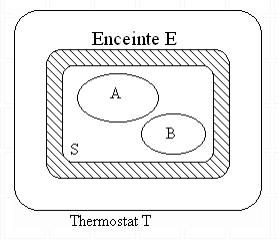
\includegraphics[scale = 0.8]{calorimetrie.png}
	\caption{Représentation schématique d'un calorimètre.} 
	\label{fig:calorimetrie}
\end{center}
\end{figure}

On veut établir le bilan énergétique du système constitué des corps A et B. On utilise pour cela le Premier Principe :
\begin{equation}
	\Delta U = \Delta U_A + \Delta U_B = W + Q = W_u + W_p + Q,
\end{equation}
où l'on a utilisé la propriété d'extensivité de l'énergie interne et où $W = W_u + W_p$ et $Q$ sont le travail et la chaleur échangés avec le milieu extérieur. $W_p$ désigne le travail des forces de pression et $W_u$ regroupe toute autre forme de travail (par exemple de l'énergie électrique provenant du secteur).\\

On travaille généralement à pression constante : la transformation est au moins monobare donc le travail des forces de pression s'écrit $W_p = - p_\text{ext}\Delta V$, d'où,
\begin{equation}
	\Delta U_A + p_\text{ext}\Delta V_A + \Delta U_B + p_\text{ext}\Delta V_B = W_u + Q,
\end{equation}
\begin{equation}
	\Delta H = \Delta H_A + \Delta H_B = W_u + Q.
\end{equation}

Il existe plusieurs types de calorimètres, notamment les calorimètres adiabatiques ($Q = 0$) et pseudo-adiabatiques (également appelés isopériboliques), pour lesquels $Q \simeq 0$.

\subsubsection{Calorimètre pseudo-adiabatique}

L'isolation thermique n'est pas parfaite et le système peut échanger de la chaleur avec le thermostat (en faible quantité). On peut négliger les transferts thermiques avec le milieu extérieur (et supposer l'enceinte calorifugée) si la durée de l'expérience est suffisamment courte devant la durée caractéristique des phénomènes de transport de la chaleur responsables des pertes thermiques du calorimètre. Ces pertes thermiques peuvent se produire sous trois grandes formes (trois modes de transport de la chaleur) :
\begin{itemize}
	\item par conduction : transfert d'agitation thermique par contact entre deux corps de température différente,
	\item par convection : transport d'énergie accompagnant un déplacement macroscopique de matière,
	\item par rayonnement : ondes électromagnétiques émises par un corps de température non nulle).
\end{itemize}
Plus de détails dans les leçons traitant des phénomènes de transport et du rayonnement thermique.\\

Plaçons nous dans les conditions où $Q \simeq 0$, d'où
\begin{equation}
	\Delta H = \Delta H_A + \Delta H_B = \simeq W_u.
\end{equation}

En supposant que A et B sont en phases condensées, le bilan enthalpique s'écrit :
\begin{equation}
	\Delta H_A + \Delta H_B = \Delta T\left[m_A c_A + C_{CAL} \right] = W_u,
\end{equation}
où $\Delta T$ désigne la variation de température subie entre l'équilibre initial et l'équilibre final et $m_A$ est la masse du corps dont on souhaite déterminer la capacité calorifique massique à pression constante $c_A$, connaissant $C_{CAL}$
\begin{equation}
	C_{CAL} = (m_B + \mu)c_B, 
\end{equation}
où $\mu$, appelée \textbf{valeur en eau} du calorimètre, est la masse d'eau à laquelle correspond la capacité calorifique du vase, de l'enceinte et des accessoires.\\

$W_u$ peut être apporté sous forme électrique : c'est le principe des méthodes électriques de calorimétrie. Un conducteur ohmique placé dans le vase calorimétrique et parcouru par un courant $I$ stationnaire fournira en un temps $\tau$ une quantité d'énergie $RI^2\tau$ qui sera absorbée par le système.\\

On présente deux calorimètres pseudo-adiabatiques \textcolor{red}[Mentionner seulement celui qui ne sera pas utilisé pour la manip. On parle de l'autre dans la section suivante] :
\begin{itemize}
	\item \textbf{Calorimètre de Berthelot} :
	
		\begin{figure}[h!]
		\begin{center}
			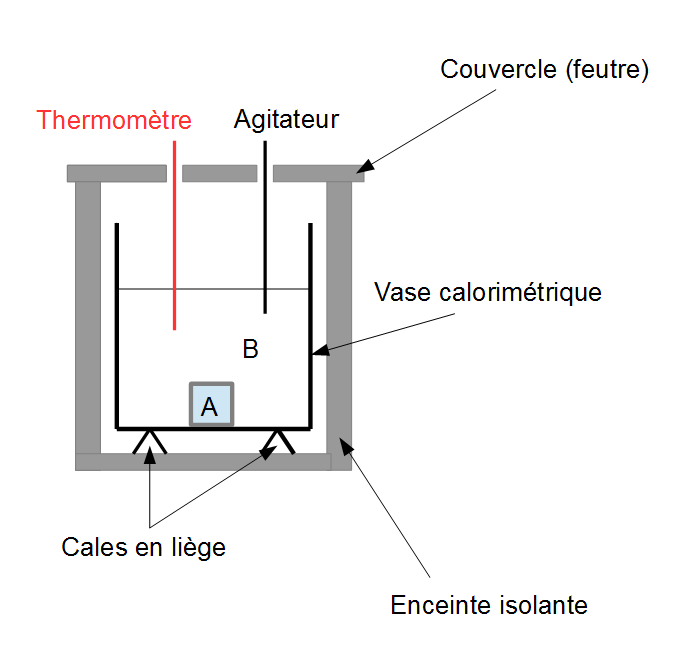
\includegraphics[scale = 0.5]{berthelot.png}
			\caption{Calorimètre de Berthelot} 
			\label{fig:berthelot}
		\end{center}
		\end{figure}
		\begin{itemize}
			\item cales en liège thermiquement isolantes
			\item parois des enceintes polies pour réduire les pertes par rayonnement
			\item feutre : bon isolant thermique\\
		\end{itemize}
		
	\item \textbf{Vase Dewar} : l'enceinte et le vase calorimétrique sont un seul et même objet
	
		\begin{figure}[h!]
		\begin{center}
			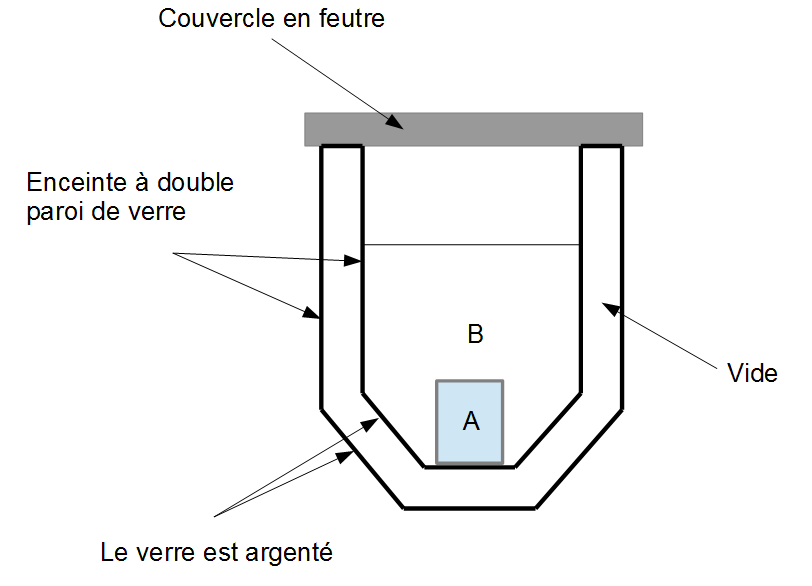
\includegraphics[scale = 0.5]{dewar.png}
			\caption{Calorimètre de Dewar} 
			\label{fig:dewar}
		\end{center}
		\end{figure}
		\begin{itemize}
			\item verre peu conducteur thermique
			\item vide : bon isolant thermique (conduction et convection faibles)
			\item parois argentées : réfléchit le rayonnement électromagnétique pour limiter les pertes par rayonnement
			\item feutre : bon isolant thermique
		\end{itemize}
\end{itemize}

Pour accélérer la thermalisation (retour à l'équilibre thermique) dans l'enceinte calorifugée, on peut introduire un agitateur (l'énergie qu'il fournit, si elle n'est pas négligeable devant $W_u$, doit être prise en compte).

\subsubsection{Mesure de la capacité calorifique du cuivre}

\textbf{Mesure de la valeur en eau du calorimètre : calorimètre + masse d'eau connue (méthode électrique)}\\

\textcolor{red}{Présenter, mais réaliser pendant la préparation.}

D'abord, étalonner la sonde/thermomètre si besoin (eau froide). Ensuite, plonger de l'eau chaude dans le calorimètre (on note toutes les températures initiales, celle de la pièce pour le calorimètre, celle de l'eau chaude). Toutes les températures doivent être mesurées avec le même appareil. Mesurer et attendre la stabilisation de la température pour relever $T_f$. Calcul pour déduire la capacité du calorimètre, convertir en masse en eau.

\begin{equation}
	C_\text{MATOS} = m_\text{eau} c_{eau} \frac{T_{eau} - T_f}{T_f - T_{ambiante}}.
\end{equation}

\textbf{Mesure de la capacité calorifique du cuivre par la méthode des mélanges}\\

On porte une masse $m_A$ de cuivre (capacité $c_A$) à la température $T_A$ dans une étuve.
On place une masse d'eau (capacité $c_B$) connue $m_B$ dans un calorimètre de masse en eau $\mu$. L'ensemble est à la température $T_\text{CAL}$.
On plonge le cuivre dans l'eau, on ferme le calorimètre et on attend que la température (thermomètre) se stabilise à une valeur $T_f$ (introduire une agitation dans l'eau accélère le processus, le transport convectif de chaleur étant plus efficace que le transport par conduction).\\

\textit{Remarque :} à l'inverse, on peut plonger le cuivre à température ambiante dans de l'eau portée à haute température (350 grammes, touiller et attendre la stabilisation).

Le calorimètre est calorifugé et on ne fournit pas de travail au système, par conséquent
\begin{equation}
	\Delta H = 0 = \Delta H_{Cu} + \Delta H_{CAL} = m_A c_A (T_f - T_A) + (m_B + \mu)c_B(T_f - T_{CAL}),
\end{equation}
d'où
\begin{equation}
	c_A = c_B \frac{m_B + \mu}{m_A}\frac{T_f - T_{CAL}}{T_A - T_f}.
\end{equation}

Les mesures doivent se faire dans les mêmes conditions que lors de l'étalonnage : même matériel, même hauteur d'eau (même surface d'échanges thermiques avec la paroi).
On doit trouver $c_p \simeq 380 \text{J.kg}^{-1}.\text{K}^{-1}$ soit $24.3 \text{J.mol}^{-1}{.K}^{-1}$ proche de la valeur mentionnée plus haut.

\textcolor{red}{Hypothèses dans le calcul :} 
\begin{itemize}
	\item constance des capacités sur la plage de température considérée (entre $T_A$ et $T_B$). Au-delà de 160 K, la capacité du cuivre obéit à Dulong et Petit. 
	\item le récipient est parfaitement calorifugé : ce n'est pas vrai, source d'erreur
\end{itemize}
\textcolor{red}{Incertitudes :}
\begin{itemize}
	\item sur $T_A$, $T_B$ et $T_F$,
	\item sur les masses $m_A$, $m_B$ et $\mu$
	\item en théorie, sur l'eau, mais on s'en sert comme référence, donc on néglige.
	\item calcul :
	\begin{equation}
		\Delta f^2 = \sum_i \frac{\partial f}{\partial x_i}^2 \Delta x_i^2
	\end{equation}
	et
	\begin{equation}
		f = f_{valeur} \pm \Delta f.
	\end{equation}
\end{itemize}

\section{Conclusion}

\end{document}